\documentclass[conference]{IEEEtran}

\usepackage[T1]{fontenc}
\usepackage{cite}
\usepackage{amsmath,amssymb,amsfonts}
\usepackage{graphicx}
\usepackage{textcomp}
\usepackage{xcolor}
\usepackage{booktabs}
\usepackage{multirow}
\usepackage{url}
\usepackage{tikz}
\usetikzlibrary{arrows.meta,positioning,fit,backgrounds,calc}

\newcommand{\pmtf}{PM\textsubscript{2.5}}
\newcommand{\notwo}{NO\textsubscript{2}}
\newcommand{\ugm}{\textmu g/m\textsuperscript{3}}
\newcommand{\rsq}{$R^2$}

\hyphenation{Open-Street-Map Light-GBM Post-GIS Map-Libre}

% Starts a new, centered row of authors.
\makeatletter
\newcommand{\linebreakand}{%
  \end{@IEEEauthorhalign}\hfill\mbox{}\par
  \mbox{}\hfill\begin{@IEEEauthorhalign}}
\makeatother

\begin{document}

\title{SIPPolusi: An End-to-End Air Pollution Exposure-Aware Routing System for Active Commuters in Jakarta}

\author{
\IEEEauthorblockN{Aurelius Justin P. F.}
\IEEEauthorblockA{\textit{School of Electrical Engineering} \\
\textit{and Informatics} \\
\textit{Institut Teknologi Bandung}\\
Bandung, Indonesia}
\and
\IEEEauthorblockN{Evelyn Yosiana}
\IEEEauthorblockA{\textit{School of Electrical Engineering} \\
\textit{and Informatics} \\
\textit{Institut Teknologi Bandung}\\
Bandung, Indonesia}
\and
\IEEEauthorblockN{Dama Dhananjaya Daliman}
\IEEEauthorblockA{\textit{School of Electrical Engineering} \\
\textit{and Informatics} \\
\textit{Institut Teknologi Bandung}\\
Bandung, Indonesia}
\linebreakand
\IEEEauthorblockN{Fedrianz Dharma}
\IEEEauthorblockA{\textit{School of Electrical Engineering} \\
\textit{and Informatics} \\
\textit{Institut Teknologi Bandung}\\
Bandung, Indonesia}
\and
\IEEEauthorblockN{Steven Tjhia}
\IEEEauthorblockA{\textit{School of Electrical Engineering} \\
\textit{and Informatics} \\
\textit{Institut Teknologi Bandung}\\
Bandung, Indonesia}
}

\maketitle

\begin{abstract}
Pedestrians and cyclists in dense cities need route guidance that accounts for air pollution, yet public monitoring networks report only at scattered stations. This paper presents SIPPolusi, an end-to-end system that converts open sensor, satellite, meteorological, and road network data into hourly street-segment exposure estimates for Jakarta, Indonesia, and serves preference-aware routes through a web application. Fine particulate matter is estimated by inverse distance weighting with a spatio-temporal graph neural network correction, and nitrogen dioxide by gradient-boosted trees. Two multi-objective reinforcement learning route policies were compared with an untrained regret heuristic and exact weighted search. Under leave-one-station-out evaluation, the nitrogen dioxide model reduced root mean square error by 41.6 percent relative to the interpolation baseline and reached a coefficient of determination of 0.71, whereas no learned fine particulate model significantly outperformed a tuned interpolator. On 200 held-out origin-destination pairs, the preference-conditioned policy reached the destination in 99.95 percent of scenarios and satisfied the requested preference on 88.5 percent of pairs, compared with 54.5 percent for a fixed-preference policy set. However, median exposure reduction against the fastest route was zero for every method, including the exact optimum, because the interpolated exposure fields offered almost no trade-off between travel time and exposure. The results indicate that the spatial structure of the exposure field, rather than the routing algorithm, is the binding constraint on exposure-aware routing in this setting.
\end{abstract}

\begin{IEEEkeywords}
air pollution exposure, active mobility, spatial downscaling, graph neural networks, multi-objective reinforcement learning, route planning
\end{IEEEkeywords}

\section{Introduction}

Air pollution imposes a substantial health and economic burden on Jakarta \cite{syuhada2023}. Pedestrians and cyclists are particularly affected because they travel slowly, breathe more deeply during physical activity, and have no cabin filtration \cite{mainka2025}. Their exposure is not fixed: field studies have shown that route type and route choice change the pollutant concentrations that commuters experience \cite{good2015,hertel2008,jarjour2013}. Acting on this finding requires pollution estimates for each street segment before a trip begins, together with a routing method that respects how much extra travel time a person is willing to accept.

Neither requirement is met by existing public services. Mainstream navigation applications optimize travel time, whereas air quality portals publish values at stations that are kilometers apart. High-resolution atmospheric modeling and commercial pollution maps can fill the gap, but they are costly or unavailable operationally in many cities. An open, reproducible pipeline from public data to route recommendations is therefore of practical interest, as is an honest measurement of what such a pipeline can deliver.

This paper describes SIPPolusi, a working prototype for Jakarta, and evaluates each of its learned components against simple baselines. The main contributions are as follows:
\begin{itemize}
\item An end-to-end system that produces hourly exposure weights for 372,069 road segments from open data, with per-pollutant fallback and a stored trace from every segment value back to its model version, input window, and grid cells.
\item A leakage-controlled comparison of spatial downscaling candidates for \pmtf{} and \notwo{}, using grouped leave-one-station-out (LOSO) validation and station-cluster bootstrap intervals.
\item A paired evaluation of two multi-objective reinforcement learning (MORL) route policies against an untrained heuristic and the exact weighted optimum on identical test scenarios.
\item Empirical evidence that smooth, station-interpolated exposure fields leave almost no time--exposure trade-off, which limits every routing method regardless of its sophistication.
\end{itemize}

\section{Related Work}

\subsection{Pollution-Aware Routing}

CAR applies A* \cite{hart1968} with a cost that combines distance and \pmtf{} concentration from ground sensors \cite{mahajan2019}. Manja \textit{et al.} merge near-real-time air quality and congestion data into an OpenStreetMap graph and search it with user-weighted A* \cite{manja2024}. Salanova Grau \textit{et al.} couple an atmospheric model and a deep-learning bias correction to a pedestrian routing engine in Thessaloniki \cite{salanova2026}. Donaldson \textit{et al.} use 10~m commercial pollution maps with graph-based routing in Leicester \cite{donaldson2026}. These systems depend on sparse point data, heavy atmospheric modeling, or paid data products.

\subsection{Spatial Downscaling}

Land-use regression relates monitored concentrations to geographic predictors \cite{hoek2008}, and machine learning has been used to downscale chemical transport models \cite{gouldsbrough2024} and to correct satellite retrievals \cite{porcheddu2024}. Spatio-temporal graph neural networks (ST-GNNs) combine temporal convolution with graph operations on sensor networks \cite{yu2018}. Evaluation requires care: random cross-validation can overstate performance when data are spatially structured, so held-out locations or blocks are needed to judge predictions at unmonitored sites \cite{roberts2017,meyer2022}.

\subsection{Multi-Objective Reinforcement Learning}

MORL learns behavior for vector-valued rewards \cite{roijers2013,hayes2022}. Preference-conditioned networks generalize across objective weights without retraining \cite{abels2019,yang2019}, whereas a fixed-preference set trains one policy per weight. When the objectives combine linearly and costs are additive, however, the problem reduces to a shortest-path search that Dijkstra's algorithm solves exactly \cite{dijkstra1959}. This exact solution is therefore the correct upper bound for any learned route policy under such an objective.

\section{System Design}

\subsection{Architecture}

Fig.~\ref{fig:architecture} shows the two-phase architecture. The background phase runs at minute 15 of every hour and processes the hour that has just ended. The real-time phase answers route requests and reads only completed cache windows, so city-wide inference never lies on the request path.

\begin{figure*}[!t]
\centering
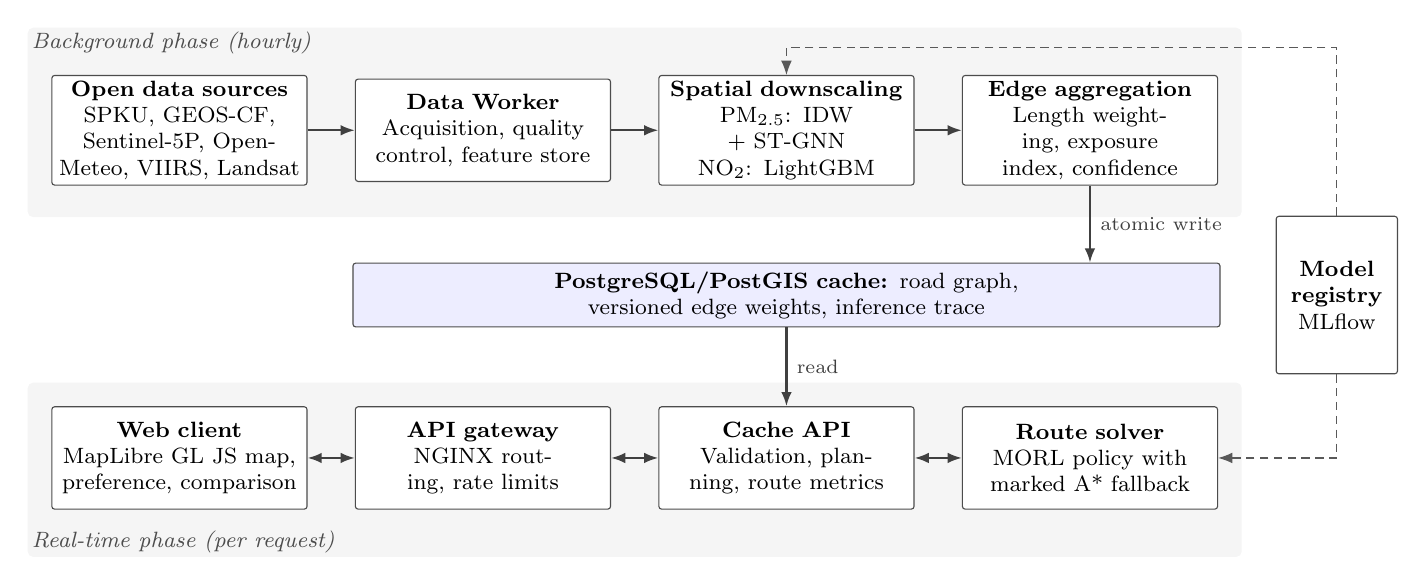
\begin{tikzpicture}[
  font=\footnotesize,
  node distance=5mm and 6mm,
  box/.style={draw=black!70, rounded corners=1pt, fill=white, align=center, text width=31mm, minimum height=13mm, inner sep=2pt},
  store/.style={draw=black!70, rounded corners=1pt, fill=blue!7, align=center, inner sep=3pt, minimum height=7mm},
  flow/.style={-{Latex[length=1.8mm]}, thick, black!75},
  both/.style={{Latex[length=1.8mm]}-{Latex[length=1.8mm]}, thick, black!75},
  dep/.style={-{Latex[length=1.8mm]}, densely dashed, black!65},
  lane/.style={fill=black!4, draw=none, rounded corners=2pt, inner xsep=3mm, inner ysep=2.5mm},
  lanelabel/.style={font=\footnotesize\itshape, text=black!70, anchor=north west, inner sep=1.5pt}
]
\node[box] (src) {\textbf{Open data sources}\\SPKU, GEOS-CF, Sentinel-5P, Open-Meteo, VIIRS, Landsat};
\node[box, right=of src] (worker) {\textbf{Data Worker}\\Acquisition, quality control, feature store};
\node[box, right=of worker] (sdm) {\textbf{Spatial downscaling}\\\pmtf: IDW + ST-GNN\\\notwo: LightGBM};
\node[box, right=of sdm] (agg) {\textbf{Edge aggregation}\\Length weighting, exposure index, confidence};

\node[store, below=10mm of $(worker.south)!0.5!(agg.south)$, text width=108mm] (cache) {\textbf{PostgreSQL/PostGIS cache:} road graph, versioned edge weights, inference trace};

\node[box, below=24mm of src |- cache.south, yshift=14mm] (client) {\textbf{Web client}\\MapLibre GL JS map, preference, comparison};
\node[box, right=of client] (gw) {\textbf{API gateway}\\NGINX routing, rate limits};
\node[box, right=of gw] (api) {\textbf{Cache API}\\Validation, planning, route metrics};
\node[box, right=of api] (solver) {\textbf{Route solver}\\MORL policy with marked A* fallback};

\node[box, text width=14mm, right=7mm of cache.east, minimum height=20mm] (reg) {\textbf{Model registry}\\MLflow};

\draw[flow] (src) -- (worker);
\draw[flow] (worker) -- (sdm);
\draw[flow] (sdm) -- (agg);
\draw[flow] (agg.south) -- node[right, font=\scriptsize] {atomic write} (agg.south |- cache.north);
\draw[flow] (api.north |- cache.south) -- node[right, font=\scriptsize] {read} (api.north);
\draw[both] (client) -- (gw);
\draw[both] (gw) -- (api);
\draw[both] (api) -- (solver);
\draw[dep] (reg.north) |- ([yshift=3.5mm]agg.north) -| (sdm.north);
\draw[dep] (reg.south) |- (solver.east);

\begin{scope}[on background layer]
\node[lane, fit=(src)(agg)(worker), inner ysep=5mm, yshift=1mm] (bg) {};
\node[lane, fit=(client)(solver), inner ysep=4.5mm, yshift=-1.5mm] (rt) {};
\end{scope}
\node[lanelabel] at (bg.north west) {Background phase (hourly)};
\node[lanelabel, anchor=south west] at (rt.south west) {Real-time phase (per request)};
\end{tikzpicture}
\caption{System architecture. The cache is the only meeting point between the hourly background phase and the per-request real-time phase. Dashed arrows show versioned model packages resolved from the registry.}
\label{fig:architecture}
\end{figure*}

The Data Worker collects station readings and secondary features, then applies quality control. Spatial models predict concentrations on a 100~m grid in EPSG:32748. Each road edge is cut at grid-cell boundaries, and its concentration for pollutant $p$ is the length-weighted mean
\begin{equation}
C_{e,p}=\frac{\sum_{g\in\mathcal{G}_e}\ell_{e,g}\,c_{g,p}}{\sum_{g\in\mathcal{G}_e}\ell_{e,g}},
\label{eq:aggregation}
\end{equation}
where $\mathcal{G}_e$ contains the cells crossed by edge $e$ that have a value for $p$, $\ell_{e,g}$ is the edge length inside cell $g$, and $c_{g,p}$ is the cell concentration.

\subsection{Exposure Definition}

\pmtf{} and \notwo{} are combined into a dimensionless index normalized by the World Health Organization 24-hour guideline values $G_{\mathrm{PM}_{2.5}}=15$ and $G_{\mathrm{NO}_2}=25$~\ugm{} \cite{who2021}:
\begin{equation}
I_e=\frac{1}{|\mathcal{P}_e|}\sum_{p\in\mathcal{P}_e}\frac{C_{e,p}}{G_p},
\label{eq:index}
\end{equation}
where $\mathcal{P}_e$ is the set of pollutants available on edge $e$. For a route $R$ with edge travel times $t_e$, travel time and cumulative exposure are
\begin{equation}
T(R)=\sum_{e\in R}t_e,\qquad E(R)=\sum_{e\in R}I_e\,t_e.
\label{eq:objectives}
\end{equation}
Travel times assume constant speeds of 1.3~m/s for walking and 4.2~m/s for cycling. $E(R)$ is an exposure proxy and not an inhaled dose.

\subsection{Reliability and Provenance}

Failures are designed to remain visible. If a model or its inputs are unavailable, that pollutant alone falls back to inverse distance weighting (IDW), and the metadata record the source and reason. Missing values are never converted to zero. A cache window becomes readable only after the edge weights and their trace are committed in one database transaction. A heuristic confidence score, $0.39\exp(-d/3000)$ for a distance $d$ in meters to the nearest sensor, is shown to users as an indicator and is not a calibrated probability.

Requests pass through an NGINX gateway that limits each client to 20 route requests per minute. The backend allots 8~s to each request. If the policy fails, times out, or returns an invalid route, the A* fastest route is returned and labeled as a fallback with the preference marked as unapplied. Model packages carry SHA-256 hashes of every file and declare their graph and data contract versions, and incompatible packages are rejected at load time.

\section{Methods}

\subsection{Dataset}

The frozen snapshot ds-v0.3.0 covers 13--30 September 2026 and the bounding box 106.68--106.98$^\circ$E, 6.38--6.08$^\circ$S. It contains 38,211 \pmtf{} and 5,372 \notwo{} station-hour labels from 105 stations, with \notwo{} measured at 14 of them. Table~\ref{tab:data} lists the sources. Quality control removes stuck sensors, sentinel values, incomplete hours, and clusters of stations reporting practically identical series, retaining 68,178 of 82,752 \pmtf{} readings and 9,863 of 10,073 \notwo{} readings. Labels are never interpolated.

\begin{table}[!t]
\caption{Data Sources}
\label{tab:data}
\centering
\footnotesize
\begin{tabular}{@{}p{0.27\columnwidth}p{0.36\columnwidth}p{0.27\columnwidth}@{}}
\toprule
\textbf{Source} & \textbf{Role} & \textbf{Resolution} \\
\midrule
SPKU stations & Labels, IDW inputs & Point, 30--60 min \\
GEOS-CF \cite{keller2021} & Analysis and forecast & 25 km, hourly \\
Sentinel-5P \cite{veefkind2012} & Tropospheric \notwo{} column & About 1.1 km (L3) \\
Open-Meteo & Meteorology & 9--11 km, hourly \\
VIIRS \cite{roman2018} & Nighttime lights & 500 m, daily \\
Landsat 8/9 & NDVI and built-up index & 30 m, 16 days \\
OpenStreetMap \cite{haklay2008} & Road graph & 373,352 edges \\
\bottomrule
\end{tabular}
\end{table}

Stations in the same grid cell, closer than 300~m, or duplicated by providers form one group, which yields 103 groups. The temporal blocks are train (13--23 September), validation (25--27 September), and test (29--30 September), separated by 25-hour gaps. Features must have been available at inference time, and all eight automated leakage checks passed on the snapshot.

\subsection{Spatial Downscaling Models}

The baseline is IDW \cite{shepard1968}, which estimates the concentration at location $x$ from station readings $y_i$ as
\begin{equation}
\hat{c}_{\mathrm{IDW}}(x)=\frac{\sum_{i\in\mathcal{N}_k(x)}d(x,x_i)^{-p}\,y_i}{\sum_{i\in\mathcal{N}_k(x)}d(x,x_i)^{-p}},
\label{eq:idw}
\end{equation}
with power $p=2$ and $k=8$ nearest stations by default.

For \pmtf{}, the deployed model adds a learned correction to this baseline,
\begin{equation}
\hat{c}_{\mathrm{PM}_{2.5}}(x)=\max\bigl(0,\ \hat{c}_{\mathrm{IDW}}(x)+\sigma\,f_\theta(x)\bigr),
\label{eq:stgnn}
\end{equation}
where $\sigma$ is the target scale and $f_\theta$ is an ST-GNN. Its 24-hour input has 58 temporal channels and passes through dilated causal temporal convolutions \cite{bai2018}. The result is fused with eight local features and refined by a two-head graph attention layer \cite{velickovic2018} on a 936-node, 4,174-edge grid graph.

For \notwo{}, the deployed model is LightGBM \cite{ke2017} with 62 features, 150 trees, and a direct concentration target. The comparison also covered kriging, Gaussian kernels, ridge regression, random forests, extra trees, XGBoost, multilayer perceptrons, regression kriging, and ensembles.

\subsection{Route Objective and Policies}

For a preference $\alpha\in[0,1]$ and $\beta=1-\alpha$, the route objective is
\begin{equation}
J_\alpha(R)=\alpha\frac{T(R)}{T_{\mathrm{ref}}}+\beta\frac{E(R)}{E_{\mathrm{ref}}},
\label{eq:objective}
\end{equation}
where $T_{\mathrm{ref}}$ and $E_{\mathrm{ref}}$ belong to the fastest route, so the fastest route always scores 1. An episode starts at the origin, and each action selects a legal outgoing arc. The scalar reward on edge $e$ is $-\alpha t_e/T_{\mathrm{ref}}-\beta I_e t_e/E_{\mathrm{ref}}$, so the return of a successful episode is $-J_\alpha(R)$. Dead ends and truncation yield a fixed return of $-4$.

The cycling graph has 299,067 nodes and 303,972 usable edges, and 26\% of its nodes have a single arc. Both policies therefore observe an ego-graph of up to 64 nodes within four hops, encoded by three message-passing layers, together with cost-to-go potentials $V_T$ and $V_E$ computed by two reverse Dijkstra searches per request. For an arc $(u,v)$, the normalized regrets, clipped to $[0,1]$, are
\begin{equation}
\begin{aligned}
\rho_T&=\bigl(t_{uv}+V_T(v)-V_T(u)\bigr)/T_{\mathrm{ref}},\\
\rho_E&=\bigl(I_{uv}t_{uv}+V_E(v)-V_E(u)\bigr)/E_{\mathrm{ref}}.
\end{aligned}
\label{eq:regret}
\end{equation}

Three candidates were compared:
\begin{itemize}
\item \textit{Fixed-preference set:} five independent actor-critic policies for $\alpha\in\{0,0.25,0.5,0.75,1\}$. A request is served by the nearest member.
\item \textit{Preference-conditioned policy:} one network with 87,043 parameters. A preference encoder modulates graph features through feature-wise linear modulation \cite{perez2018}, and the arc logit is $g_\phi(\cdot)-\lambda(\alpha\rho_T+\beta\rho_E)$ with a learned scale $\lambda$.
\item \textit{Regret prior:} an untrained baseline that greedily minimizes $\alpha\rho_T+\beta\rho_E$.
\end{itemize}

Training used imitation of exact weighted routes for 400 episodes, followed by proximal policy optimization (PPO) \cite{schulman2017}. It drew from 2,000 training origin--destination (OD) pairs of 0.5--3~km and 17 training time windows, and 75\% of episodes used synthetically perturbed exposure fields. Checkpoints were selected on validation data. For the preference-conditioned policy, PPO did not improve validation return, so the selected checkpoint is the imitation warm start.

\subsection{Evaluation Protocol}

\textit{Spatial models:} The primary protocol is grouped LOSO on the test block. Each held-out group is excluded from training, normalization, and all sensor-derived features, and model selection uses the validation block. Uncertainty is reported with a 95\% station-cluster bootstrap \cite{cameron2008} of the RMSE difference from baseline, using 4,000 resamples. The design targets are \rsq{}~$\geq0.60$ with RMSE at least 10\% below baseline on held-out test data, and \rsq{}~$\geq0.50$ at unseen locations.

\textit{Route models:} The primary test set has 200 OD pairs of 0.5--3~km whose endpoints lie in spatial blocks unused in training, seven test time windows, and 11 values of $\alpha$, giving 2,200 scenarios. Exposure comes from hourly IDW fields. The research targets are a median exposure reduction of at least 4\% at $\alpha=0.5$ with at most 20\% added time, and preference fulfillment on at least 80\% of OD pairs. A pair is fulfilled when moving from $\alpha=1$ to $\alpha=0$ neither raises exposure nor lowers travel time. Identical routes satisfy this definition, so the share of pairs that actually shift route is reported beside it. The evaluation protocol was committed before the test split was first read for the fixed-preference set. The paired comparison reused those scenarios and is therefore exploratory.

\section{Results}

\subsection{Spatial Downscaling}

Table~\ref{tab:spatial} and Fig.~\ref{fig:forest} summarize the LOSO results. For \notwo{}, LightGBM reduced RMSE from 46.99 to 27.43~\ugm{}, a reduction of 41.6\% (difference $-19.56$, 95\% CI $[-29.74, -10.40]$), and improved all 13 test stations. Its pooled \rsq{} of 0.71 meets the design targets.

\begin{table}[!t]
\caption{Pooled LOSO Test Results (RMSE and MAE in $\mu$g/m$^3$). Bold Marks the Deployed Model for Each Pollutant}
\label{tab:spatial}
\centering
\footnotesize
\setlength{\tabcolsep}{3.2pt}
\begin{tabular}{@{}lrrrrrr@{}}
\toprule
& \multicolumn{3}{c}{\pmtf{} ($n=4{,}358$)} & \multicolumn{3}{c}{\notwo{} ($n=604$)} \\
\cmidrule(lr){2-4}\cmidrule(l){5-7}
\textbf{Method} & RMSE & MAE & \rsq{} & RMSE & MAE & \rsq{} \\
\midrule
IDW ($p=2$, $k=8$) & 24.00 & 17.32 & $-0.04$ & 46.99 & 38.81 & 0.14 \\
IDW ($p=1$, all) & 22.18 & 16.32 & 0.11 & 45.55 & 37.45 & 0.19 \\
Ordinary kriging & 22.26 & 16.31 & 0.11 & 52.85 & 40.53 & $-0.09$ \\
LightGBM (all feat.) & 22.95 & 16.67 & 0.05 & \textbf{27.43} & \textbf{20.74} & \textbf{0.71} \\
IDW + ST-GNN & \textbf{23.74} & \textbf{17.86} & $\mathbf{-0.02}$ & 47.17 & 33.10 & 0.13 \\
\bottomrule
\end{tabular}
\end{table}

\begin{figure*}[!t]
\centering
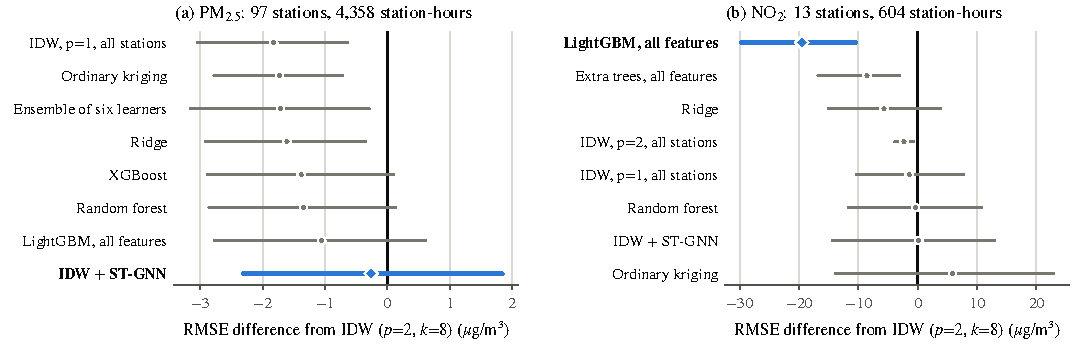
\includegraphics[width=\textwidth]{figures/spatial_forest.pdf}
\caption{RMSE difference from the IDW baseline under LOSO, with 95\% station-cluster bootstrap intervals. Negative values favor the listed method. Blue diamonds and bold labels mark the deployed model for each pollutant.}
\label{fig:forest}
\end{figure*}

For \pmtf{}, no learned model was significantly better than a tuned interpolator. IDW with $p=1$ and all stations, the configuration selected on the validation block, achieved an RMSE of 22.18~\ugm{}, which is 7.6\% below the default baseline. The deployed IDW + ST-GNN model achieved 23.74~\ugm{}; its difference from the baseline was not significant (95\% CI $[-2.31, +1.85]$), and it was significantly worse than tuned IDW (95\% CI of the difference $[+0.27, +2.98]$). On the separate fixed split of 689 station-hours, it lowered RMSE from 18.74 to 18.37~\ugm{} (95\% CI of the difference $[-0.58, -0.10]$), a statistically significant improvement of only 2.0\%. The \pmtf{} design targets were not met.

Variance diagnostics explain this outcome. On the training block, persistent station offsets account for 54\% of \pmtf{} variance, the shared hourly level for 14\%, and the station-hour remainder for 32\%. The offsets are stable over time, with a correlation of 0.87 between the training and test blocks, yet neighboring stations do not predict them (correlation $-0.04$), and neither do the available covariates (LOSO \rsq{}~$\leq0$).

The \notwo{} gain comes mainly from sensor-geometry features. With the same hyperparameters, LightGBM achieved an RMSE of 47.04~\ugm{} on interpolation features alone, 29.82~\ugm{} after adding geometry, and 47.29~\ugm{} using all features except geometry. Distance to the nearest \notwo{} station and local sensor density contribute 34\% and 27\% of the model's gain importance. These features separate a high-reading central cluster that includes low-cost sensors from peripheral government stations. Low-cost sensors are known to require careful calibration \cite{karagulian2019}, so part of this gain may reflect network bias and should not be assumed to transfer across the city grid.

\subsection{Route Policies}

Table~\ref{tab:routes} reports the primary test results. All candidates passed the validity, success, and latency gates. The preference-conditioned policy met the preference target with 88.5\% fulfillment, whereas the fixed-preference set reached 54.5\%. At $\alpha=0.5$ it matched the exact optimum on 141 of 200 pairs, compared with 89 for the fixed-preference set.

\begin{table}[!t]
\caption{Route Results on 200 Held-Out OD Pairs With IDW Fields}
\label{tab:routes}
\centering
\footnotesize
\setlength{\tabcolsep}{2.6pt}
\begin{tabular}{@{}lrrrrr@{}}
\toprule
\textbf{Metric} & \textbf{Target} & \textbf{Fixed} & \textbf{Cond.} & \textbf{Prior} & \textbf{Exact} \\
\midrule
Route success (\%) & $\geq95$ & 100 & 99.95 & 99.50 & 100 \\
Returned routes valid (\%) & 100 & 100 & 100 & 100 & 100 \\
Inference p95 (ms) & $\leq4500$ & 362 & 377 & 285 & n/m \\
Median exposure cut (\%) & $\geq4$ & 0.00 & 0.00 & 0.00 & 0.00 \\
Median added time (\%) & $\leq20$ & 0.10 & 0.00 & 0.00 & 0.00 \\
Preference fulfilled (\%) & $\geq80$ & 54.5 & 88.5 & 100 & 100 \\
Pairs with shifted route (\%) & -- & 8.0 & 15.0 & 24.0 & 24.0 \\
Same route as exact$^{\mathrm{a}}$ & -- & 89 & 141 & 189 & 200 \\
Mean objective gap$^{\mathrm{a}}$ (\%) & -- & 0.53 & 0.04 & 0.04 & 0 \\
\bottomrule
\end{tabular}

\vspace{2pt}
\parbox{\columnwidth}{\scriptsize $^{\mathrm{a}}$At $\alpha=0.5$; the prior reached 198 of 200 destinations. Fixed: fixed-preference set. Cond.: preference-conditioned policy. Prior: regret prior. n/m: not measured.}
\end{table}

No method achieved the exposure target. The median exposure reduction at $\alpha=0.5$ was 0.00\% for every method, including the exact optimum. The optimum saved at least 4\% on only 3 of 200 pairs, and its mean saving was 0.23\% at $\alpha=0.5$ and 0.38\% at $\alpha=0$. Fig.~\ref{fig:tradeoff}(a) shows how little trade-off the IDW fields contain. The target was thus unreachable on these fields by any routing method.

\begin{figure*}[!t]
\centering
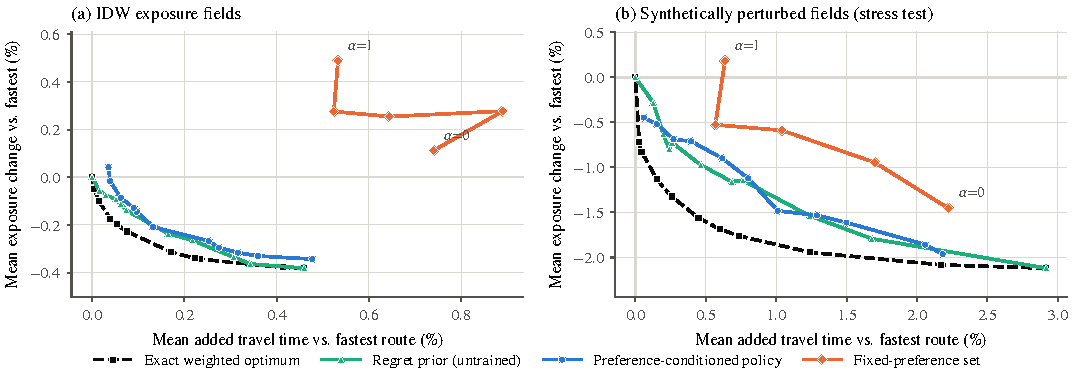
\includegraphics[width=\textwidth]{figures/route_tradeoff.pdf}
\caption{Mean paired change against the fastest route as the preference moves from $\alpha=1$ to $\alpha=0$, across 200 OD pairs and reached routes only. Lower and further left is better. Perturbed fields are synthetic and do not indicate real-world exposure savings.}
\label{fig:tradeoff}
\end{figure*}

The untrained regret prior performed about as well as the trained preference-conditioned policy, with the same 0.04\% objective gap and 100\% preference fulfillment, although it failed more often (99.50\% against 99.95\% success). Most routing quality therefore comes from the two exact cost-to-go searches. On the synthetic perturbed fields, the conditioned policy fulfilled 91.0\% of preferences and shifted route on 36.2\% of pairs, against 61.6\% and 19.2\% for the fixed-preference set and 100\% and 46.5\% for the optimum. On longer 3--8~km trips, which lie outside the training range, the conditioned policy succeeded on 98.5\% of decoded routes and the fixed-preference set on 93.2\%.

\subsection{System Verification}

A controlled end-to-end suite passed all 64 checks, covering empty caches, unavailable data sources, solver timeouts, malformed responses, database outages, and false-success detection. That suite uses IDW and a stub route model, as shown in Fig.~\ref{fig:client}. In a separate local replay with both registered spatial models, no cell used the fallback. Model inference took 315~s, road aggregation 79~s, and the cache write 38~s, producing weights for 372,069 of 373,352 edges (99.66\%). A request through the local gateway then returned a policy route with the preference applied.

\begin{figure}[!t]
\centering
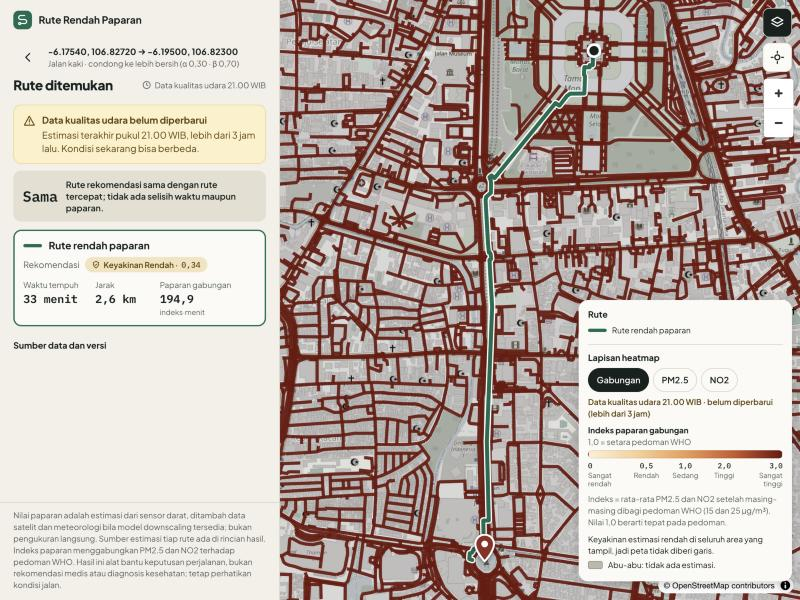
\includegraphics[width=\columnwidth]{figures/web_client.jpg}
\caption{Web client (Indonesian interface) in the controlled end-to-end test. The recommended route equals the fastest route, and the interface states this along with stale-data and low-confidence notices instead of implying a saving.}
\label{fig:client}
\end{figure}

A Google Cloud deployment also serves the web application end to end, and one cycling request through its public gateway completed in about 1.3~s. That deployment currently uses the fixed-preference policy set and IDW pollution estimates, because the registered spatial model packages have not yet been transferred to it. Sustained latency, availability, and usability have not yet been measured.

\section{Discussion}

\textit{The exposure field bounds the routing benefit.} IDW produces smooth surfaces between stations, and in a representative hourly window the median grid cell lay 1.7~km from its nearest station. Alternative routes between the same OD pair therefore pass through nearly identical estimated concentrations. Even a perfect optimizer cannot create a saving that the field does not contain. Evaluating routing against the exact optimum made this limit visible; a comparison with the fastest route alone would have attributed the failure to the policy.

\textit{Exact search remains the appropriate default for this objective.} Because \eqref{eq:objective} is additive over edges for fixed reference values, weighted Dijkstra search returns the optimum and cannot dead-end. A learned policy can match it at best, and the evaluated policies already execute two exact searches per request. MORL may still be useful for non-additive objectives or tighter latency budgets, but this study did not measure the runtime of weighted search and provides no evidence of such an advantage.

\textit{Better \pmtf{} estimates likely require better measurements.} Persistent offsets that neither neighbors nor covariates explain suggest instrument calibration or very local siting effects. Added model capacity is unlikely to recover them. The deployed IDW + ST-GNN pairing is an implementation choice that differs from the evaluation's recommendation of tuned IDW.

\textit{Threats to validity.} The dataset spans 18 days in a single season, and each model was trained with one random seed. The spatial test results had been inspected during development, so they are exploratory. Route evaluation used IDW fields and not the registered spatial models, so the trade-off available under those models remains unknown. MORL policies were trained for cycling only, and walking requests receive the marked A* fallback. Constant speeds ignore signals, congestion, and slope. Station-level accuracy does not establish accuracy across the 100~m grid.

\section{Conclusion}

SIPPolusi demonstrates that open data can be turned into traceable, hourly street-segment exposure weights and preference-aware routes for Jakarta. Its \notwo{} model achieved a substantial gain at held-out stations, with the caveat that the gain depends on sensor geometry. Its \pmtf{} models did not significantly surpass a tuned interpolator. The preference-conditioned route policy followed user preferences more reliably than a fixed-preference set, but no method reduced median exposure on interpolated fields, including the exact optimum.

Future work should repeat the route evaluation on fields from the registered models, calibrate or flag low-cost sensors, and extend the dataset across seasons. It should also benchmark weighted search as a production alternative and complete load and usability testing. The source code and experiment records are available at \url{https://github.com/ppthimmel/SIPPolusi}.

\section*{Acknowledgment}

This work was carried out in the IF5200 Applied Research Project course at Institut Teknologi Bandung, taught by Dessi Puji Lestari and Robithoh Annur. The authors acknowledge the Jakarta Environmental Agency and the providers of the open data used in this study.

% Balances the two columns of the last page; readjust if the content changes.
\IEEEtriggeratref{23}

\bibliographystyle{IEEEtran}
\bibliography{references}

\end{document}
